\documentclass[12pt]{article}
\usepackage{amssymb, amsmath}
\usepackage{fancyhdr,lastpage}
\usepackage{amsmath,amsfonts,amssymb}
\usepackage{graphicx}
\usepackage{stix}
\usepackage{enumitem}
\usepackage{listings}
\usepackage{float}
\tolerance 10000
\headheight 0in
\headsep 0in
\evensidemargin 0in
\oddsidemargin \evensidemargin
\textwidth 6.5in
\topmargin .25in
\textheight 8.7in

\usepackage{listings}
\usepackage{color}
 
\definecolor{codegreen}{rgb}{0,0.6,0}
\definecolor{codegray}{rgb}{0.5,0.5,0.5}
\definecolor{codepurple}{rgb}{0.58,0,0.82}
\definecolor{backcolour}{rgb}{0.95,0.95,0.92}
 
\lstdefinestyle{mystyle}{
    backgroundcolor=\color{backcolour},   
    commentstyle=\color{codegreen},
    keywordstyle=\color{magenta},
    numberstyle=\tiny\color{codegray},
    stringstyle=\color{codepurple},
    basicstyle=\footnotesize,
    breakatwhitespace=false,         
    breaklines=true,                 
    captionpos=b,                    
    keepspaces=true,                 
    numbers=left,                    
    numbersep=5pt,                  
    showspaces=false,                
    showstringspaces=false,
    showtabs=false,                  
    tabsize=2
}

\lstset{style=mystyle}

\newcommand{\CC}{{\mathbb C}}
\newcommand{\QQ}{{\mathbb Q}}
\newcommand{\RR}{{\mathbb R}}
\newcommand{\ZZ}{{\mathbb Z}}
\newcommand{\NN}{{\mathbb N}}
\newcommand{\FF}{{\mathbb F}}


\newcommand{\Zerobold}{{\boldsymbol 0}}
\newcommand{\Onebold}{{\boldsymbol 1}}
\newcommand{\xbold}{{\boldsymbol x}}

\newcommand{\mfrak}{{\mathfrak m}}

\newcommand{\Acal}{{\mathcal A}}
\newcommand{\Ncal}{{\mathcal N}}
\newcommand{\Pcal}{{\mathcal P}}
\newcommand{\Qcal}{{\mathcal Q}}

\newcommand{\sqbinom}[2]{\genfrac{[}{]}{0pt}{}{#1}{#2}}
\newcommand{\angbinom}[2]{\genfrac{\langle}{\rangle}{0pt}{}{#1}{#2}}

\newcommand{\qddx}{(d/dx)_{q}}

%\newcommand{\pfcl}{\emph{Proof of claim}}
\newenvironment{proof}{\paragraph{Proof: }}{\hfill$\blacksquare$}



\def\multiset#1#2{\ensuremath{\left(\kern-.3em\left(\genfrac{}{}{0pt}{}{#1}{#2}\right)\kern-.3em\right)}}


\DeclareMathOperator{\des}{des}
\DeclareMathOperator{\maj}{maj}
\DeclareMathOperator{\ev}{ev}
\DeclareMathOperator{\Hom}{Hom}
\DeclareMathOperator{\trace}{tr}
\DeclareMathOperator{\inv}{inv}

\newtheorem{problem}{Problem}%[section]

\begin{document}

\begin{center}
{\bf Julio Soldevilla}
\\
{\bf EECS 504 Winter 2018 --- Problem Set 2}
\end{center}

\begin{problem}
\normalfont
Problem1
\end{problem}

\begin{proof}
\begin{enumerate}

\item For an image of the given size $n \times n$ and a Gaussian kernel of size $(2k+1) \times (2k+1)$, when we apply the kernel to just one full window in the image, we have $(2k+1)^2$ multiplications and $(2k+1)^2-1$ additions. Then, to go over the whole picture, we need to make the convolution with $(n-(2k+1)+1)^2$ windows, and so this implies that in total the total number of operations to convlve the imgabe by the kernel is $(n-2k)^2 * ((2k+1)^2 + (2k+1)^2 -1)$.

\item Consider the $2D$ Gaussian kernel $G_{2D}(s,t) = \frac{1}{2\pi\sigma^2}e^{-\frac{s^2+t^2}{2\sigma^2}} = \frac{1}{\sqrt{2\pi}\sigma}e^{-\frac{s^2}{2\sigma^2}} \times \frac{1}{\sqrt{2\pi}\sigma}e^{-\frac{t^2}{2\sigma^2}} = G_{1D}(s)\times G_{1D}(t)$ where we define $\frac{1}{\sqrt{2\pi}\sigma}e^{-\frac{s^2}{2\sigma^2}}  = G_{1D}(s)$ and $\frac{1}{\sqrt{2\pi}\sigma}e^{-\frac{t^2}{2\sigma^2}} = G_{1D}(t)$ are the 1D Gaussian Kernel's. Then, if we convolve $G_{2D}(s,t)$ with some function $f$, we have that $G_{2D}(s,t)*f = (G_{1D}(s)\times G_{1D}(t))*f = G_{1D}(s)\times(G_{1D}(t)*f)$ and we see that convolving with 2D Gaussian is the same as convolving with 1D Gaussian twice. 

\item Replacing the $2D$ Gaussian kernel with the 1d Gaussian kernel would imply that for applying the 1D horizontal kernel to one window of the corresponding size we would do $(2k+1)$ multiplications and $2k$ additions. Then, we can do this operation in a row for $(n-2k)$ times and then we need to repeat this process $n$ times. So, we end up having to do $n(n-2k)[(2k+1) + 2k]$ operations for applying the horizontal 1D Gaussian Kernel. Then, we will have the exact same count of operations for the vertical 1D Gaussian Kernel. Thus, for applying the 1D Gaussian Kernel twice we would have to do $2n(n-2k)[(2k+1)+2k]$ operations. \\

In the case of a 2D kernel of $5 \times 5$, applying the 2D kernel we would need $(n-4)^2 *49$ operations to convolve the image with the kernel. Applying the 1D kernel twice we would need $18n(n-4)$ operations. Then, we can see that there will definitely be some $n$ such that applying the $2D$ kernel is cheaper. TO figure out the exact amount, we just set the equations equal and find the value of $n$. Doing this, we et $n = \frac{196}{31} \approx 6.3$ Thus, when $n \geq 7$, it is cheaper to apply the $1D$ Gaussian Kernel twice instead of the $2D$ Kernel.

\item Now, recall that the LoG operator is given by the mask: $\left[ \begin{matrix}  0 & -1 & 0 \\ -1 & 4 & -1 \\ 0 & -1 & 0\end{matrix} \right]$ or $\left[\begin{matrix}  -1 & -1 & -1 \\ -1 & 8 & -1 \\ -1 & -1 & -1\end{matrix} \right]$. For a Kernel to be separable, we must be able to find two vectors whose outer product is the kernel shown above, which is the same as saying that the rows of the matrix representing the kernel are linearly dependent. We can clearly see that this is not the case in the LoG and so we conclude that the LoG is not separable. \\

Recall we can approximat ethe LoG with Difference of Gaussians. One thing we can do to ahiceve an almost equivalent operation as if using LoG is to do a difference of 2D Gaussians and use the separability of this operator to get a cheaper operator than using the LoG but still with similar results.

\item Finally, let $\left[\begin{matrix} u' \\ v' \end{matrix} \right] = \left[\begin{matrix} \cos(\theta) & -\sin(\theta) \\ \sin(\theta) & \cos(\theta) \end{matrix} \right] \left[\begin{matrix} u \\ v \end{matrix} \right]$. Notice that \begin{equation} u'^2 = u^2(\cos^2(\theta)) - 2uv\cos(\theta)\sin(\theta) + v^2 \sin^2(\theta) \end{equation} and \begin{equation} v'^2 = u^2(\sin^2(\theta)) + 2uv\cos(\theta)\sin(\theta) + v^2 \cos^2(\theta) \end{equation}. Then we have that $(G_1 - G_2)(u',v') = G_1(u',v') - G_2(u',v') = \frac{1}{2\pi \sigma_1^2} e^{-\frac{u'^2 + v'^2}{2\sigma_1^2}} - \frac{1}{2\pi \sigma_2^2} e^{-\frac{u'^2 + v'^2}{2\sigma_2^2}} \stackrel{\text{by eq. 1 and 2}}{=} \frac{1}{2\pi \sigma_1^2} e^{-\frac{u^2 + v^2}{2\sigma_1^2}} - \frac{1}{2\pi \sigma_2^2} e^{-\frac{u^2 + v^2}{2\sigma_2^2}} = G_1(u,v) - G_2(u,v)$. Thus, this shows that the DoG operator is rotationally invariant, as desired.

\end{enumerate}
\end{proof}

\begin{problem}
\normalfont
Problem 2
\end{problem}

\begin{proof}
\begin{enumerate}

\item The code for harris is the following:

\lstinputlisting[language=Matlab]{harris.m}

The output images are:

\begin{figure}[H]
\begin{center}
\advance\leftskip-3cm
\advance\rightskip-3cm
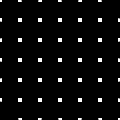
\includegraphics[keepaspectratio=true, scale = 1]{response_checkerboard.png}
\caption{}
\label{visina8}
\end{center}
\end{figure}

\begin{figure}[H]
\begin{center}
\advance\leftskip-3cm
\advance\rightskip-3cm
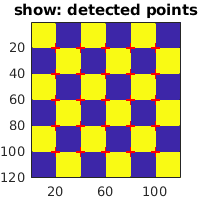
\includegraphics[keepaspectratio=true, scale = 1]{detect_checkerboard.png}
\caption{}
\label{visina8}
\end{center}
\end{figure}

\item

Running run\_3\_2.m generates the following image:

\begin{figure}[H]
\begin{center}
\advance\leftskip-3cm
\advance\rightskip-3cm
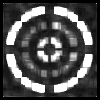
\includegraphics[keepaspectratio=true, scale = 1]{response_rings.png}
\caption{}
\label{visina8}
\end{center}
\end{figure}

This image looks like this because the original image is not completely smooth, so the Harris detector is actually detecting this non smoothness of the figure. The Harris detector is considering the brusque changes in the intensity of the pixels forming the image as corners of the circles and so that is why there are so many responses in the picture. Since the image is not smooth (in terms of changes of intensities in the pixels) the detector has a response for places that are not in the circles. No full ring has a high corner response over the entire ring, because when we are in the north, south, east and west parts of the circles, the pixels of very similar intensity  are  exactly stacked one over the other or one next to the other and so for this small regions of the circles there are no brusque changes in the values of the pixels and so in these regions, the operator doesn't detect these regions as corners and the output doesn't show a high corner response in this part. 

\item The code we use for this function is

\lstinputlisting[language=Matlab]{run_3_3.m}

The image this changed code generates is:

\begin{figure}[H]
\begin{center}
\advance\leftskip-3cm
\advance\rightskip-3cm
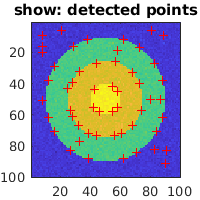
\includegraphics[keepaspectratio=true, scale = 1]{detect_rings.png}
\caption{}
\label{visina8}
\end{center}
\end{figure}

In this code, we can see that the Harris operator detected corners only on the boundaries. This happens because in the detect function in the write up, change false to true makes the program convolve the image with a Gaussian smoothing kernel that will smooth the corner-like features that were detected before by the Harris operator. 

\item The code script run\_red\_varyk.m returns the following six images:

\begin{figure}[H]
\begin{center}
\advance\leftskip-3cm
\advance\rightskip-3cm
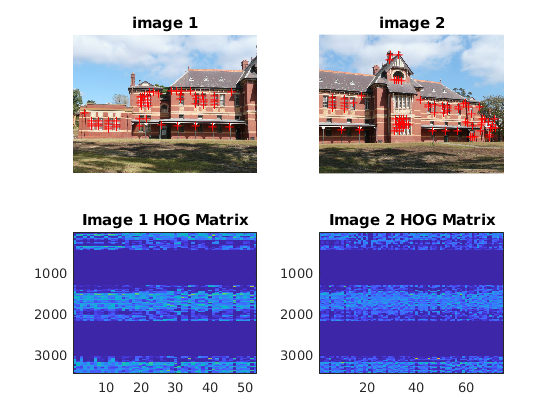
\includegraphics[keepaspectratio=true, scale = 1.3]{red_showcorrespondences_4.png}
\caption{Red correspondences with 4 points}
\label{visina8}
\end{center}
\end{figure}

\begin{figure}[H]
\begin{center}
\advance\leftskip-3cm
\advance\rightskip-3cm
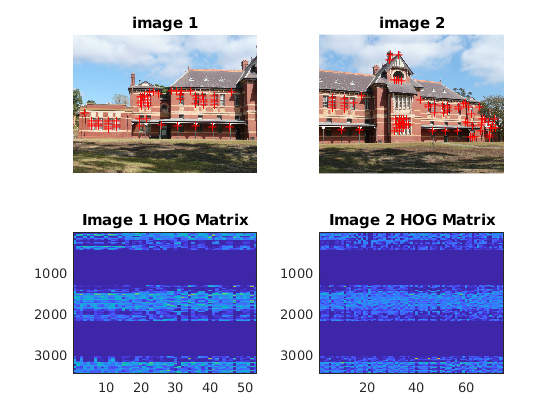
\includegraphics[keepaspectratio=true, scale = 1.3]{red_showcorrespondences_10.png}
\caption{Red correspondences with 10 points}
\label{visina8}
\end{center}
\end{figure}

\begin{figure}[H]
\begin{center}
\advance\leftskip-3cm
\advance\rightskip-3cm
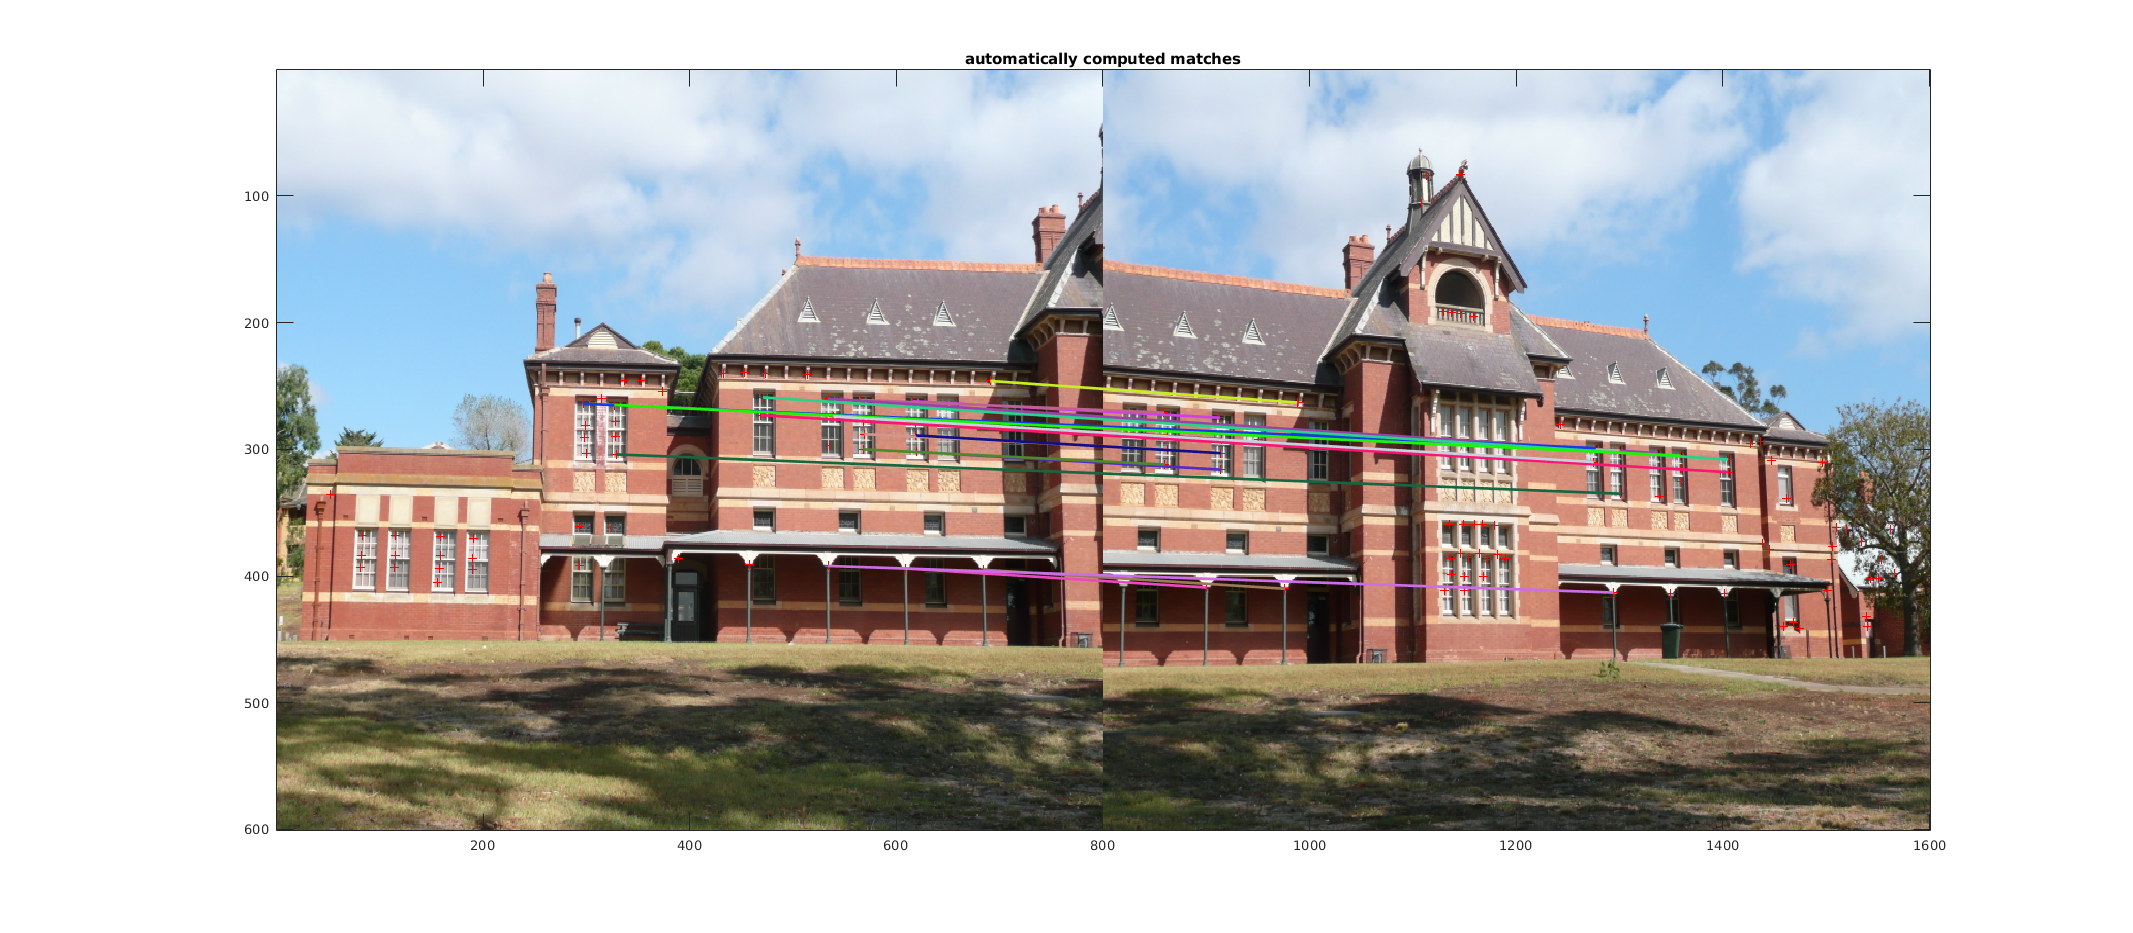
\includegraphics[keepaspectratio=true, scale = 0.3]{red_showcorrespondences_20.png}
\caption{Red Correspondences with 20 points.}
\label{visina8}
\end{center}
\end{figure}

\begin{figure}[H]
\begin{center}
\advance\leftskip-3cm
\advance\rightskip-3cm
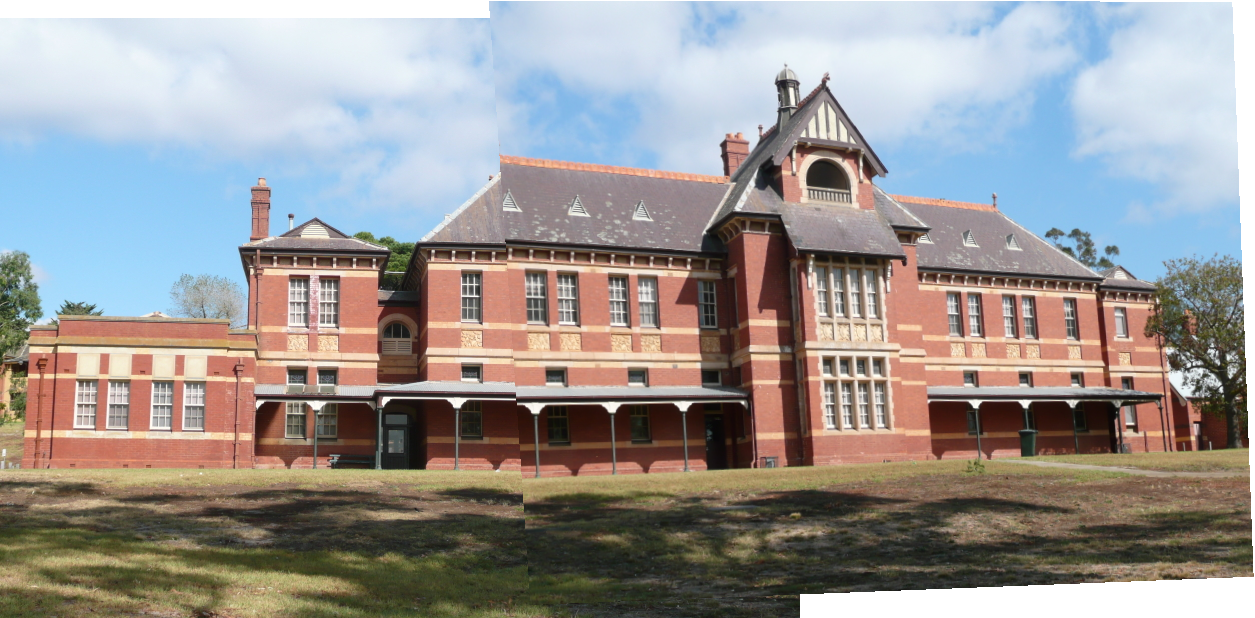
\includegraphics[keepaspectratio=true, scale = 0.5]{red_stitched1_4.png}
\caption{Red stichted with 4 points.}
\label{visina8}
\end{center}
\end{figure}

\begin{figure}[H]
\begin{center}
\advance\leftskip-3cm
\advance\rightskip-3cm
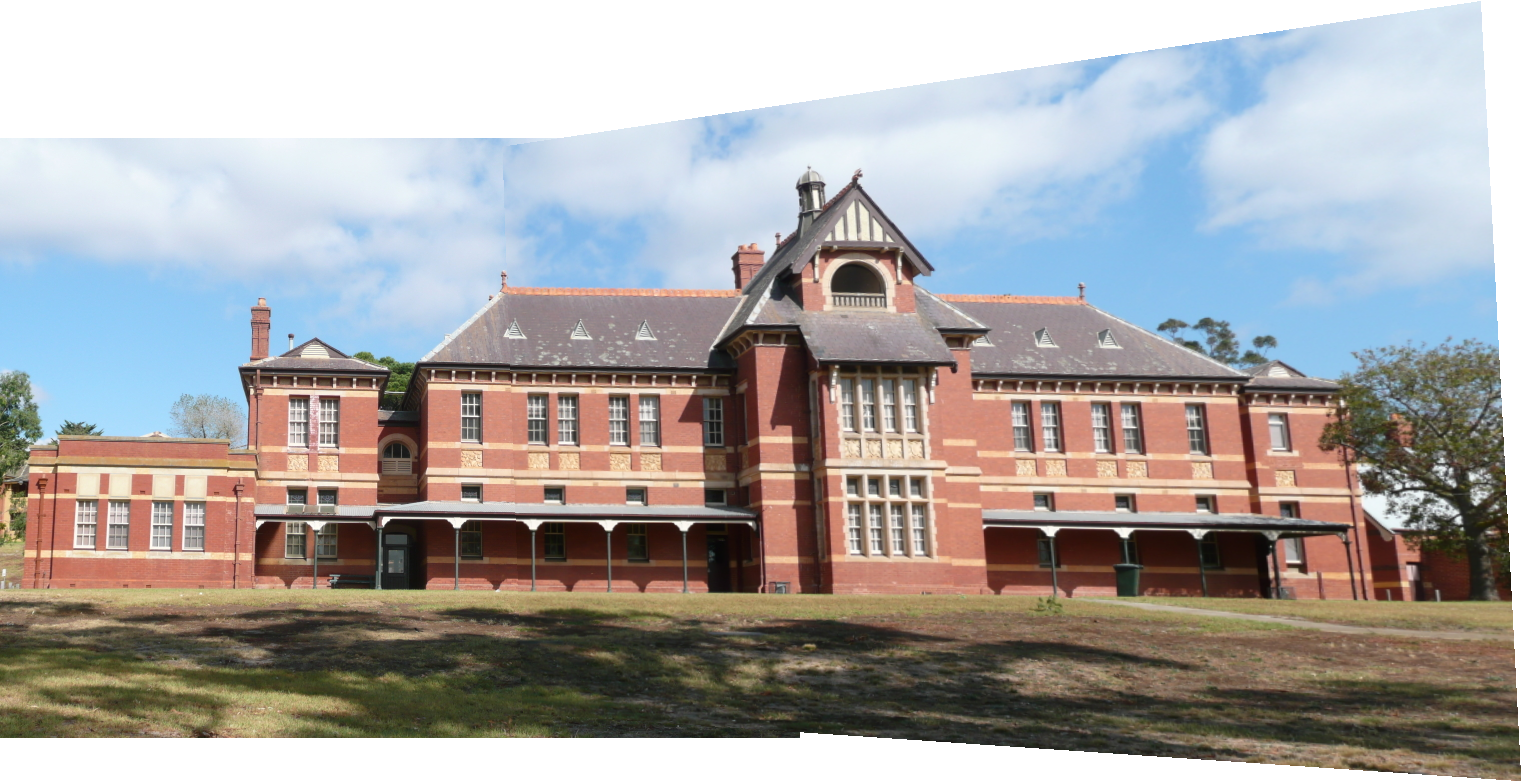
\includegraphics[keepaspectratio=true, scale = 0.5]{red_stitched1_10.png}
\caption{Red stichted with 10 points.}
\label{visina8}
\end{center}
\end{figure}

\begin{figure}[H]
\begin{center}
\advance\leftskip-3cm
\advance\rightskip-3cm
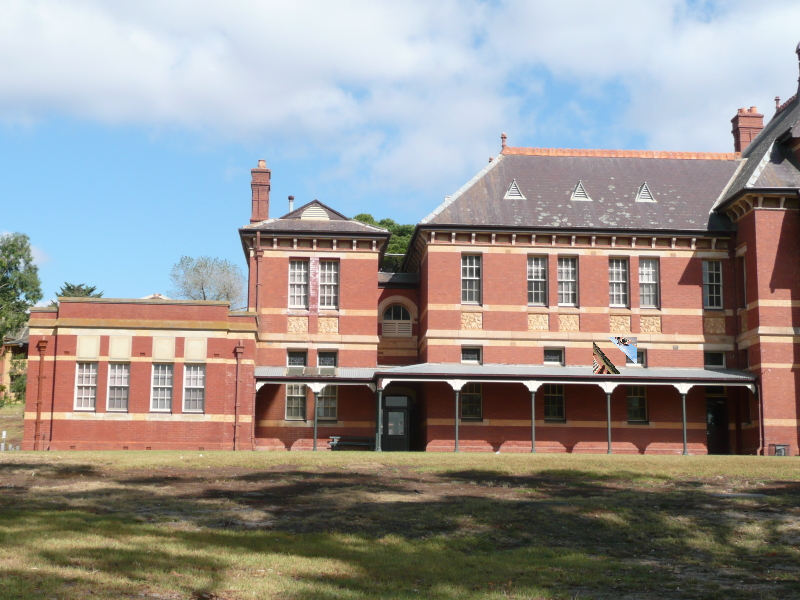
\includegraphics[keepaspectratio=true, scale = 0.5]{red_stitched1_20.png}
\caption{}
\label{Red stichted with 20 points}
\end{center}
\end{figure}

IN this case, we can see that the best correspondence comes when we use 10 points. This happens because with 10 points there is information to match the picture correctly and therefore the estimation is optimal. When we have only 4 points, we don't have enough points to match the pictures adequately and so the estimation is not accurate, that is why we end up having the picture shown above. Finally, with 20 points, we now have too much information, namely too many points, and so the code cannot process so much information and ends up mismatching the points and therefore there is a wrong estimation of the homography that aligns the image. 

\end{enumerate}
\end{proof}

\pagebreak
\begin{problem}

Problem 3

\end{problem}

\begin{proof}
\begin{enumerate}
\item The DoG Scale space for the circle is the following:

\begin{figure}[H]
\begin{center}
\advance\leftskip-3cm
\advance\rightskip-3cm
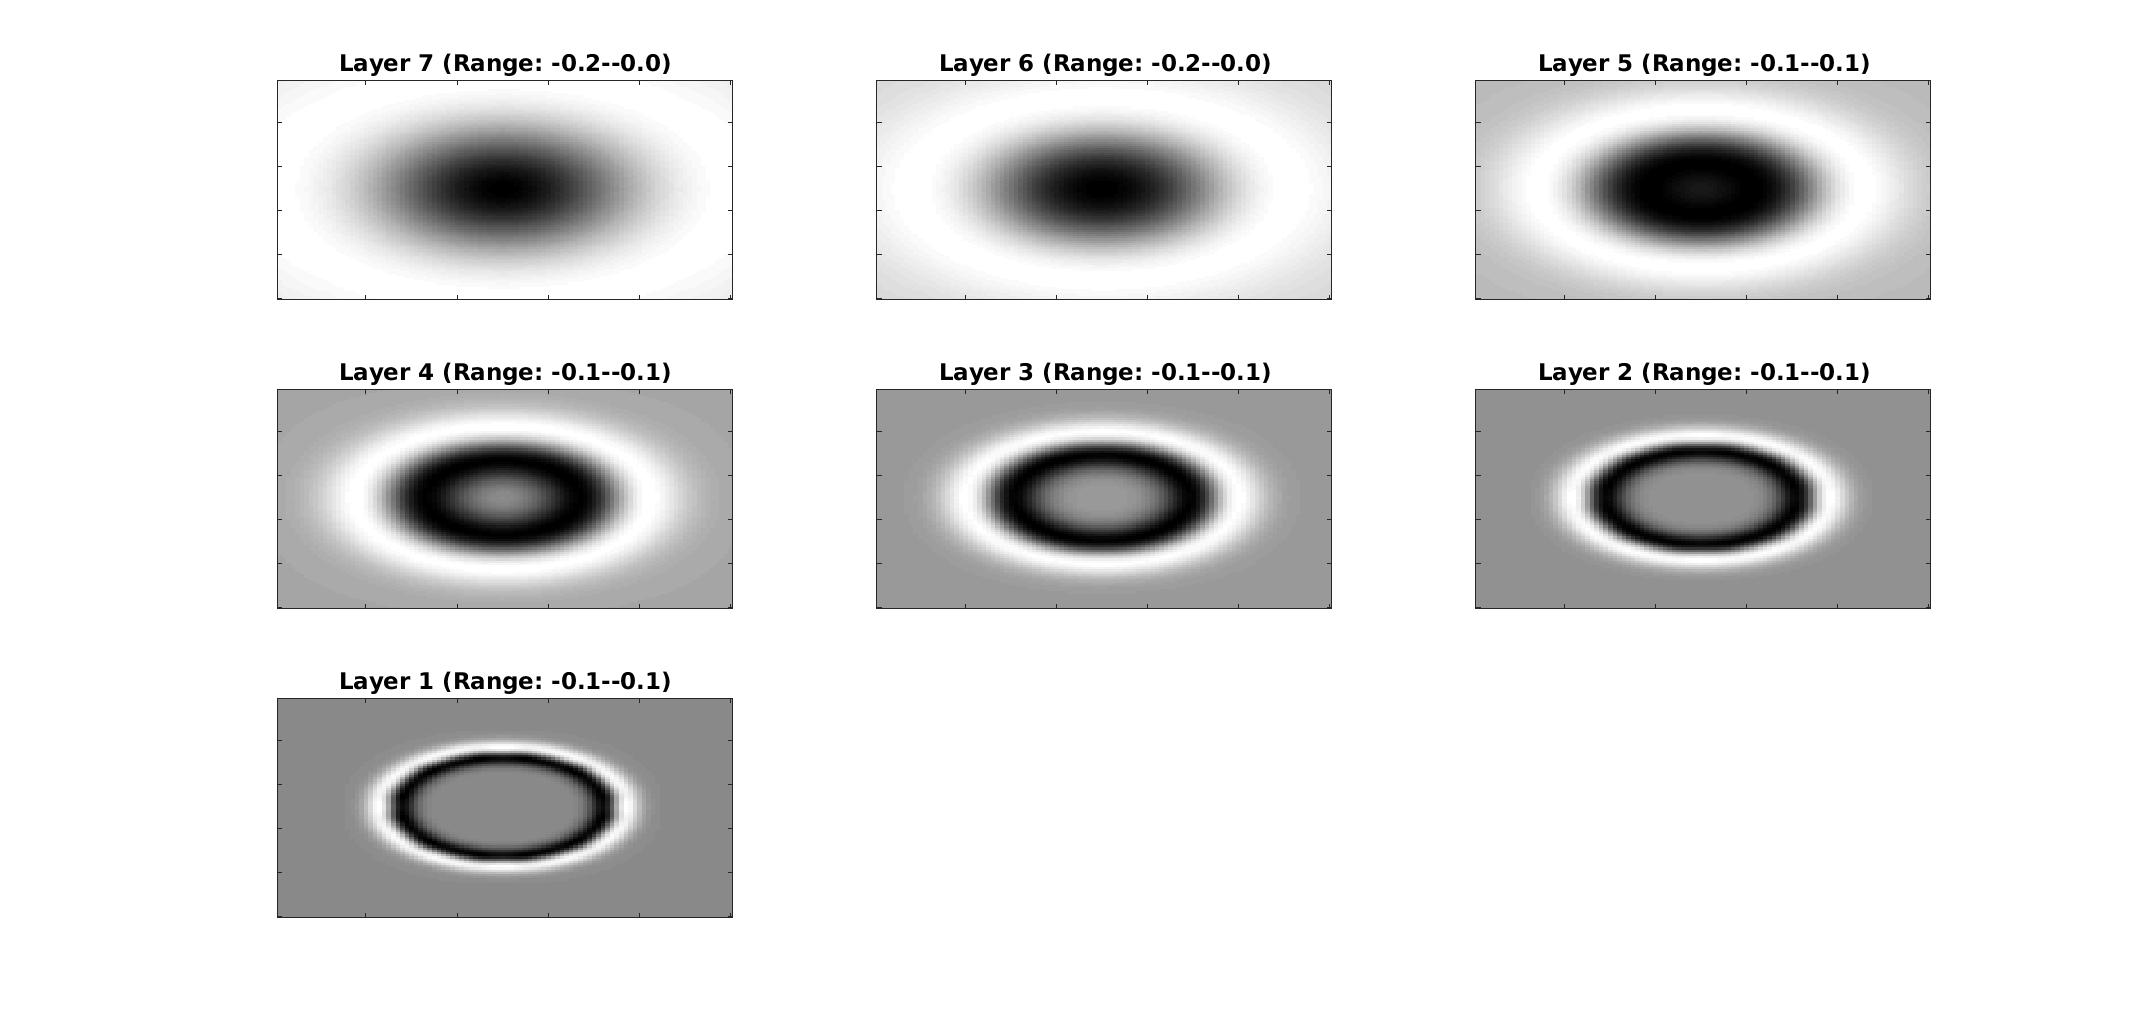
\includegraphics[keepaspectratio=true, scale = 0.2]{circle_scale_space.jpg}
\caption{}
\label{Circle scale space}
\end{center}
\end{figure}

The scale space for the sunflower picture is:

\begin{figure}[H]
\begin{center}
\advance\leftskip-3cm
\advance\rightskip-3cm
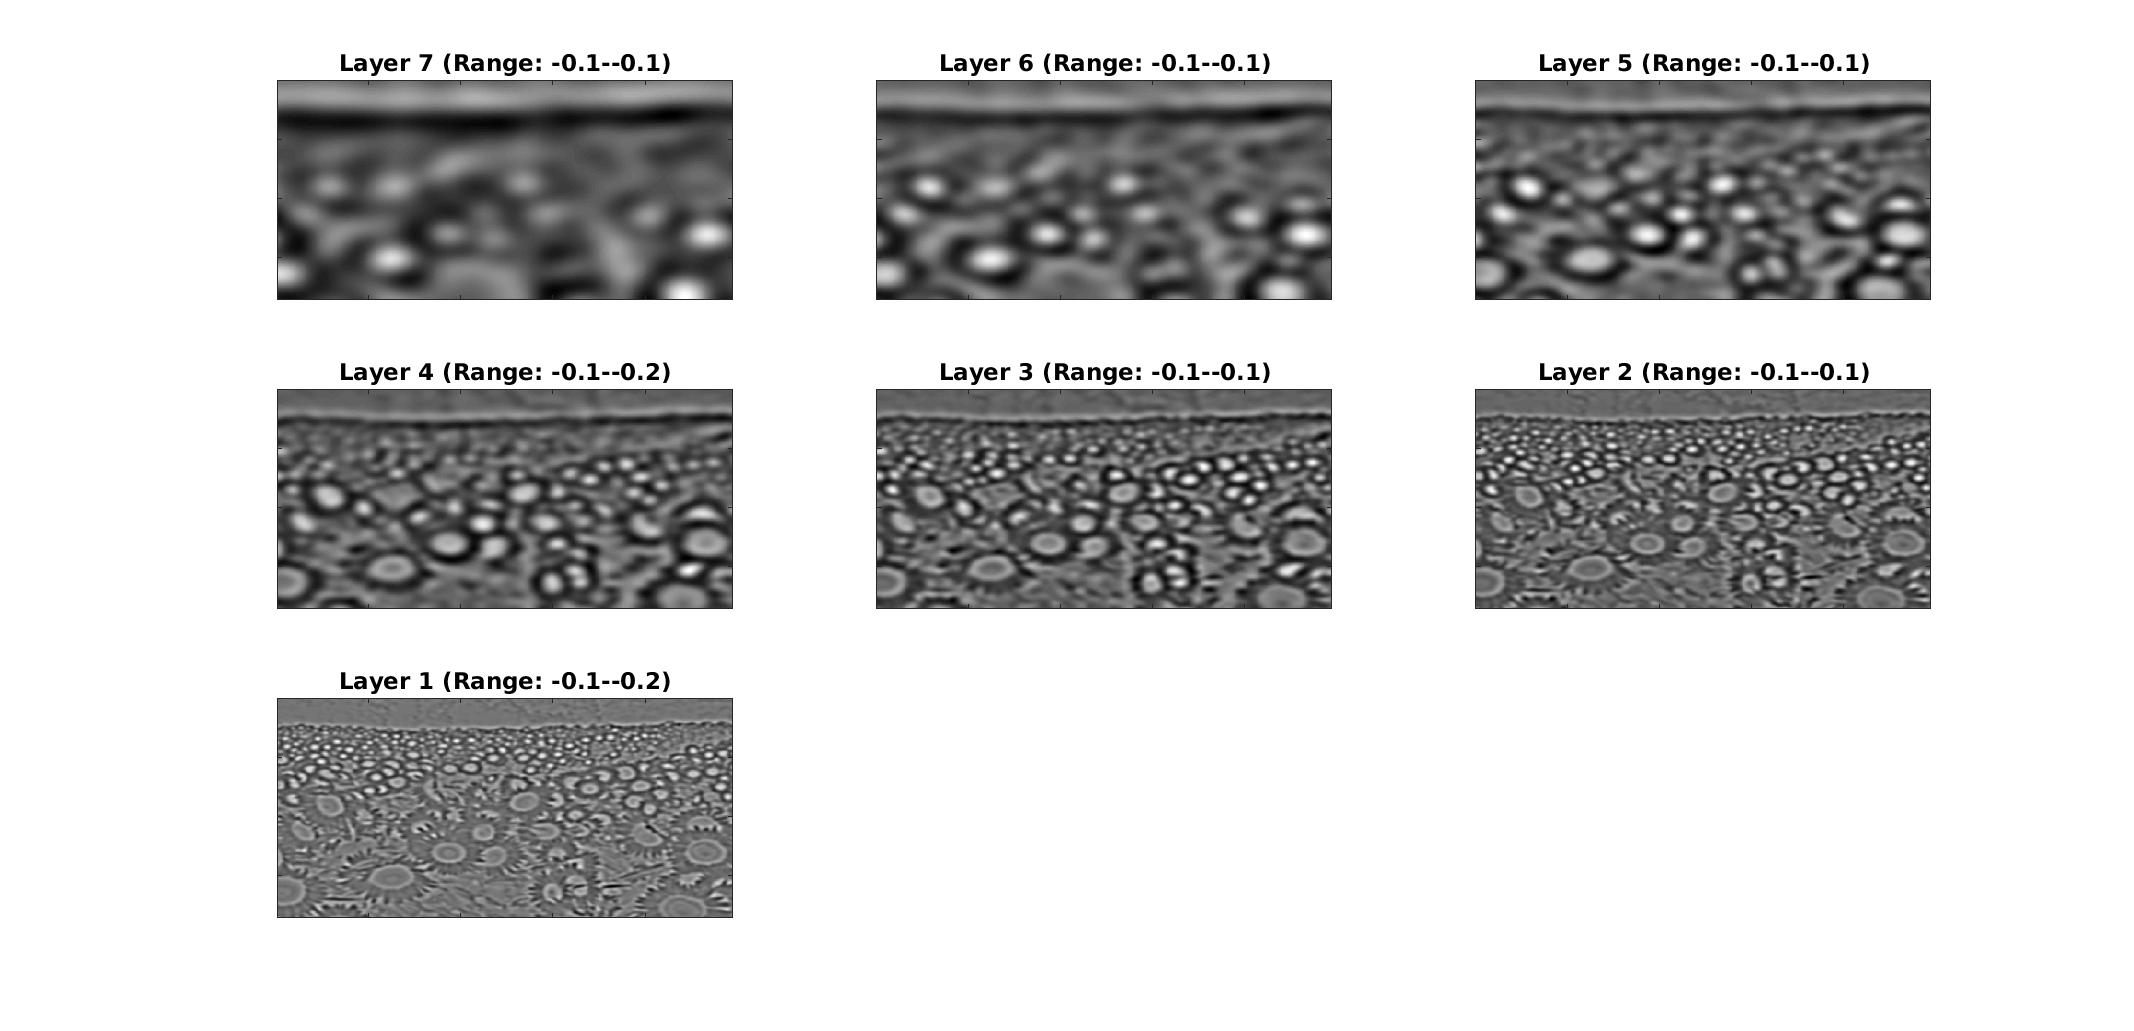
\includegraphics[keepaspectratio=true, scale = 0.2]{sunflower_scale_space.jpg}
\caption{}
\label{Sunflower Scale space}
\end{center}
\end{figure}

THe fly brain scale space picture is:

\begin{figure}[H]
\begin{center}
\advance\leftskip-3cm
\advance\rightskip-3cm
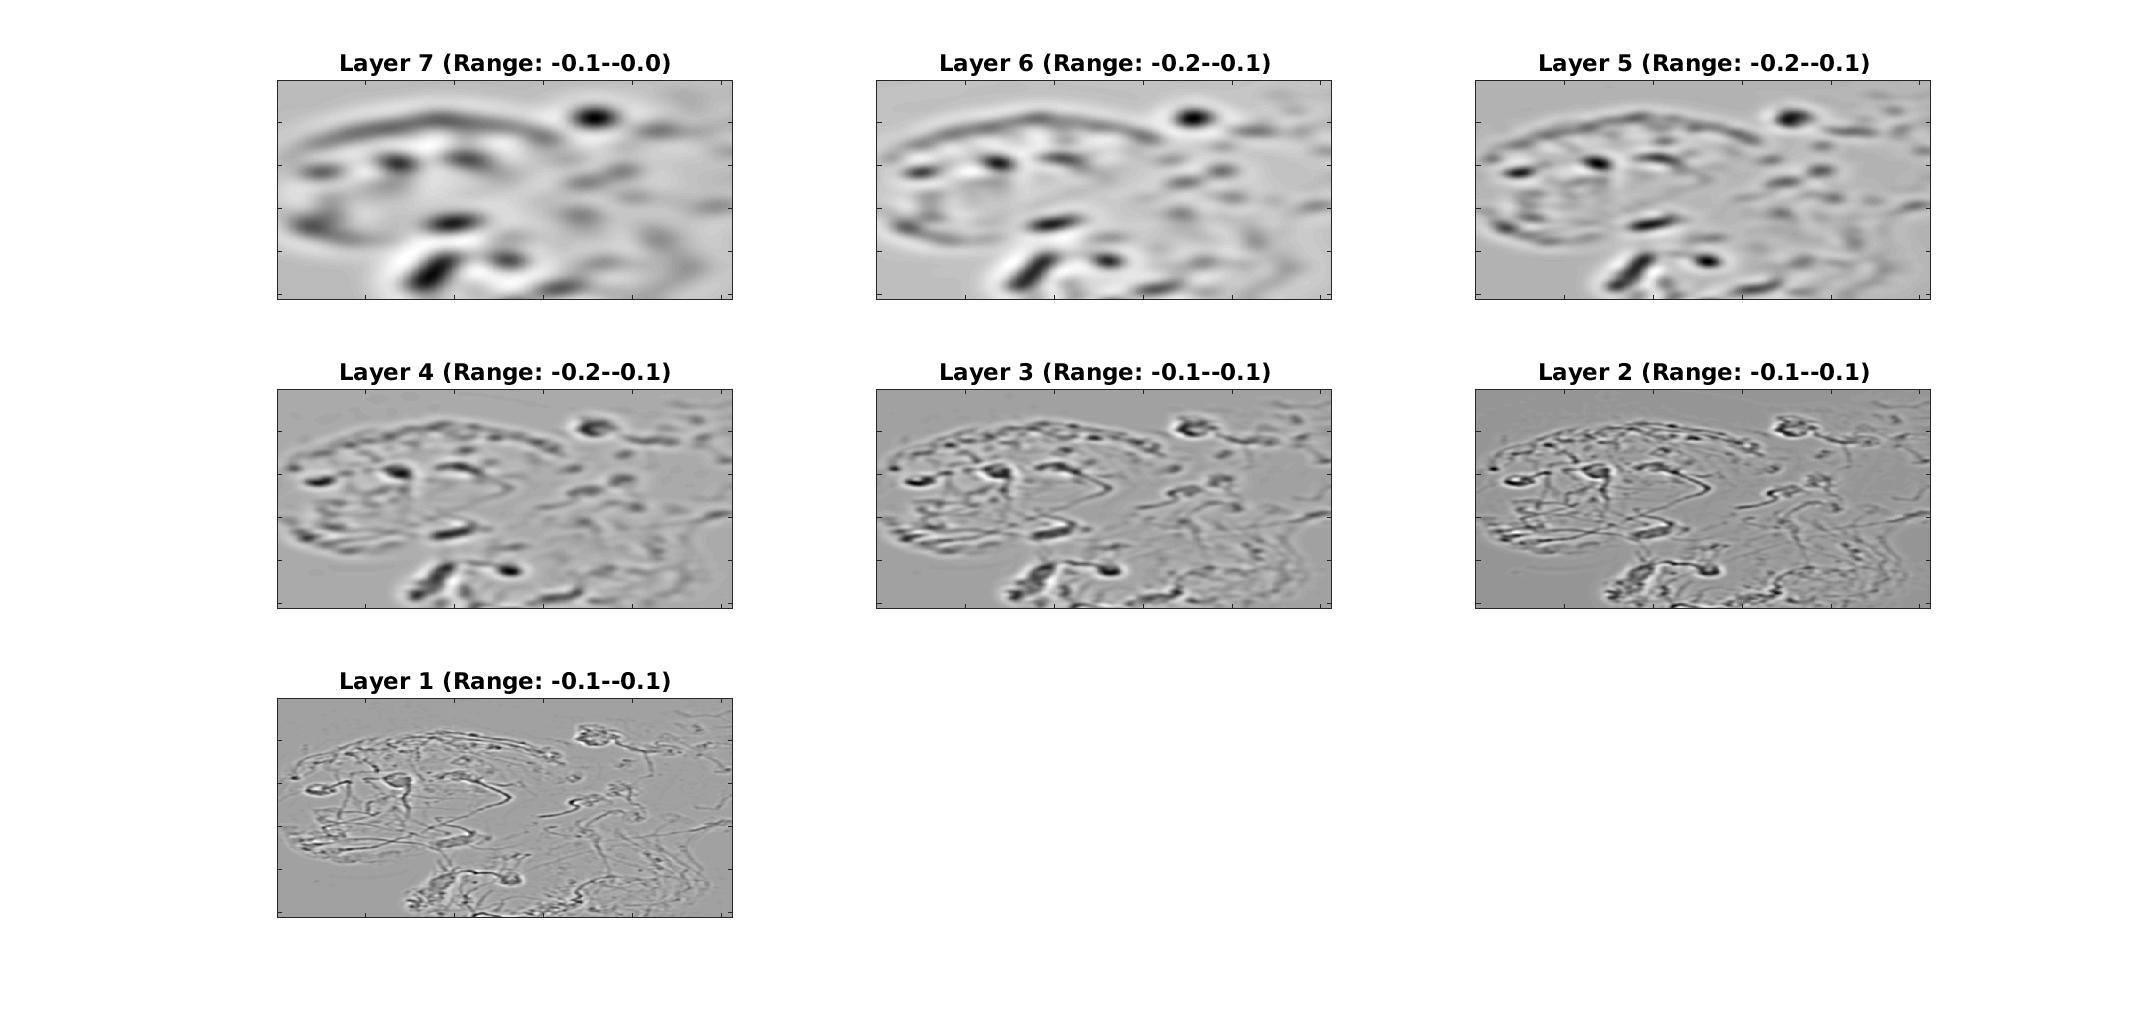
\includegraphics[keepaspectratio=true, scale = 0.2]{fly_scale_space.jpg}
\caption{}
\label{Fly Scale Space}
\end{center}
\end{figure}

In the sunflower scale space we can see how the how the centers of the sunflowers are always recognizable, even after blurring in the 7th layer of the DoG scale. A similar thing happens with the circle scale space, which is just a much simpler space than the sunflower space. In the circle space, it is interesting to see how the outer and inner part of the circle are almost of the same color in layer 1, but as we increase in the layers, the center of the circle turns white, the edge becomes whiter and bigger and we see almost nothing of the outside of the edge by layer 7. 

\item In the following pictures, we have the visualization of the detected extrema.

\begin{figure}[H]
\begin{center}
\advance\leftskip-3cm
\advance\rightskip-3cm
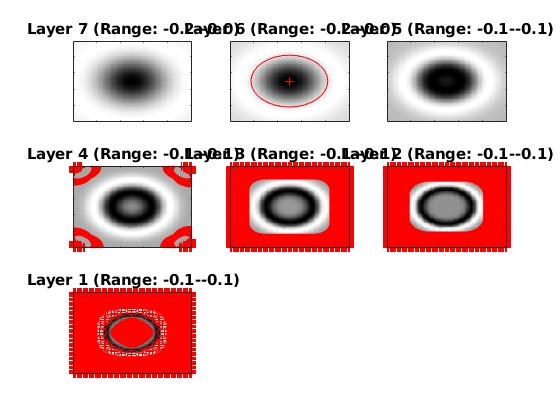
\includegraphics[keepaspectratio=true, scale = 1.2]{circle_maxima.jpg}
\caption{}
\label{Circle maxima}
\end{center}
\end{figure}

the visualization of fly maxima is:

\begin{figure}[H]
\begin{center}
\advance\leftskip-3cm
\advance\rightskip-3cm
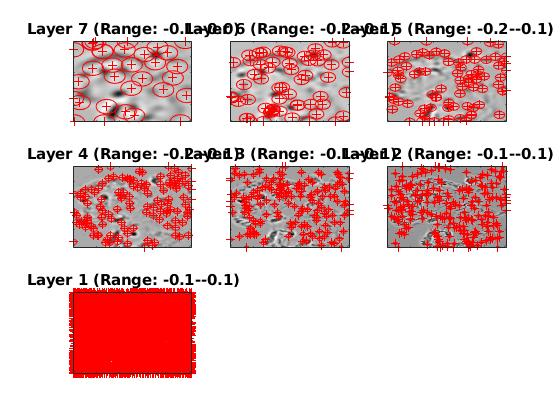
\includegraphics[keepaspectratio=true, scale = 1.2]{fly_maxima.jpg}
\caption{}
\label{Fly maxima visualization}
\end{center}
\end{figure}

The visualization of sunflower maxima:

\begin{figure}[H]
\begin{center}
\advance\leftskip-3cm
\advance\rightskip-3cm
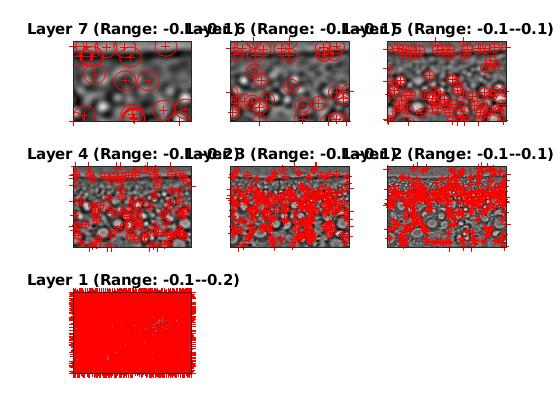
\includegraphics[keepaspectratio=true, scale = 1.2]{sunflower_maxima.jpg}
\caption{}
\label{Sunflower maxima visualization}
\end{center}
\end{figure}

So in the pictures above, we detect many extrema in the first layers, because in these layers, the $\sigma$ of the Gaussian is small and so, thinking about the picture of the Gaussian, this is very narrow. Thus, there is a lot of variation in neighboring pixels and this leads us to detect in regions with even small variations a lot of points as maxima and minima points. As the $\sigma$ increases, the Gaussian is wider and so there is less brusque variation in neighboring pixels, which implies we will have fewer and fewer maxima and minima. As a ressult, we will detect fewer and fewer maxima and minima in larger regions. That is why we detect less blobs and detect them over wider regions. 


\item As a filtering idea, after doing the threshold filtering, I wanted to take the points in the picture corresponding to the remaining detected blobs and take them as center of windows (of size similar to the radius of the blob) and use these windows to compute the Structure tensor to compute the minimum eigenvalue of such a tensor. In this way, I would be able to detect whether there were any corners in the blob centered at the point we picked. If there were corners, we can discard that blob because we want blobs, not corners. And so going through all the points represented in the vector of maxima found in part 2 of the problem, we would filter even more the blobs.

The code is the following:


\lstinputlisting[language=Matlab]{filterBlobs.m}

The picture of the sunflowers after filtering blobs is :

\begin{figure}[H]
\begin{center}
\advance\leftskip-3cm
\advance\rightskip-3cm
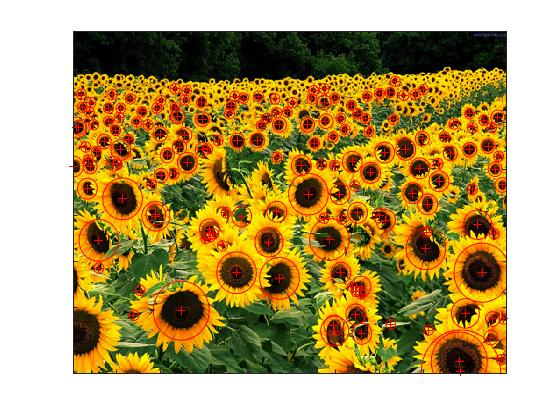
\includegraphics[keepaspectratio=true, scale = 0.8]{filtered_sunflower.jpg}
\caption{}
\label{Fltered sunflowers}
\end{center}
\end{figure}

\begin{figure}[H]
\begin{center}
\advance\leftskip-3cm
\advance\rightskip-3cm
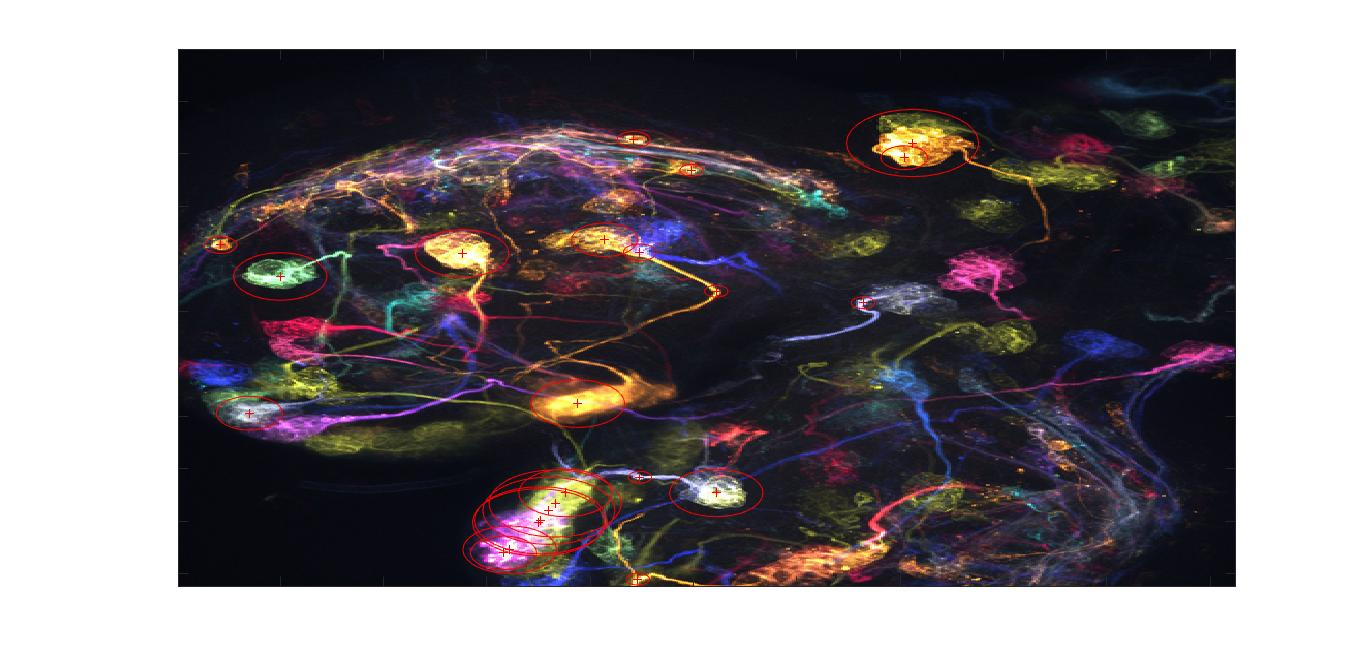
\includegraphics[keepaspectratio=true, scale = 0.4]{filtered_brainfly.jpg}
\caption{}
\label{Filtered brainfly}
\end{center}
\end{figure}

\begin{figure}[H]
\begin{center}
\advance\leftskip-3cm
\advance\rightskip-3cm
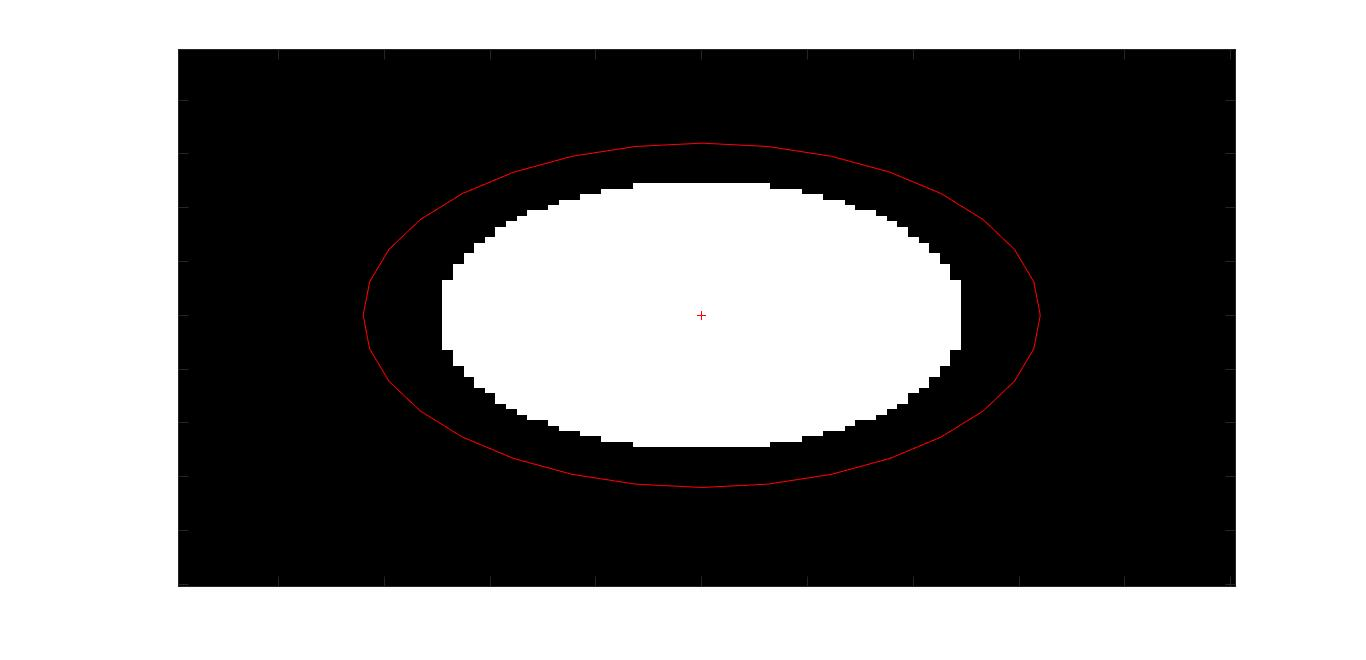
\includegraphics[keepaspectratio=true, scale = 0.4]{filtered_circle.jpg}
\caption{}
\label{Filtered Circle}
\end{center}
\end{figure}


\end{enumerate}
\end{proof}


\end{document}